\chapter{Results and Discussion} 
\label{chp:results}
In this chapter, we present the results of the experiments described in Chapter~\ref{chp:experiments} and discuss the performance of the models.
First, in Section~\ref{sec:test-data-results}, we describe the development, training and testing split of the dataset.
Then, we present the results of the graph combination model and discuss the most important features of the logistic regression classifier.
Moreover, we compare it to the performance of the iterative models in the same test dataset and explain the shortcoming of the graph combination model.
Second, we display the results of the iterative models using the entire \wikirfa dataset in Section~\ref{sec:complete-reults}.
Further, we examine the performance of the iterative models and discuss the optimal selection of threshold to predict results.
Lastly, the results of the voting order experiments are presented in Section~\ref{sec:voting-order-results}.
We analyse the significance of the voting order on the performance of the iterative models.


\section{Test Dataset Results}
\label{sec:test-data-results}

\begin{table}[htp]
    \centering
    \caption{\wikirfa dataset split information}
    \label{tab:data-splits}
    \begin{tabular}{lcccc}
        \toprule
        Feature & Development & Training & Testing \\
        \midrule

        Percentage &30\% & 30\% & 40\% \\
        Number of votes & 62833 & 62807 & 83830 \\
        Number of RfAs &1668& 1551&1314 \\
        First Date &22/02/2004 & 31/10/2006 &24/06/2008 \\
        Last Date &06/11/2006& 30/06/2008 & 01/01/2019
        \\  
        

        \bottomrule
        \end{tabular}
\end{table}

\begin{itemize}
    \item Discuss the data splits
    \item The number of RfAs and votes in each split
    \item Explain the small overlap in first and last dates
    \item Show the results table and explain the baselines 
\end{itemize}

\begin{table}[htp]
    \centering
    \caption{Results of different models for the test split of the \wikirfa dataset}
    \label{tab:test-results}
    \begin{tabular}{lccc}
        \toprule
        Model & AUC-ROC & \aucposPR  & \aucnegPR \\ 
        \midrule
        
        Baseline & 0.5 & 0.776 & 0.224 \\

        Graph Combination &  0.542 & 0.798 & 0.251 \\

        Iterative Balance &  0.815 & 0.922 & 0.614 \\

        Iterative Status & 0.754 & 0.9 & 0.486 \\
        
        \bottomrule
        \end{tabular}
\end{table}

\subsection{Graph Combination Model results}


\begin{table}[htp]
    \centering
    \caption{Information of graphs formed using development data split}
    \label{tab:test-results}
    \begin{tabular}{lcccc}
        \toprule
        Graph & $|G|$ & $\|G\|$ & density & \shortstack{size of \\largest  component} \\ 
        \midrule
        
        Similarity Graph & 6368 &1463465 & 0.0721 & 6368 \\
        
        Talk Graph & 5477 & 213307 & 0.0071 & 3489 \\

        Signed Graph & 4675 & 65595 & 0.003 & 1083 \\

        \bottomrule
        \end{tabular}
\end{table}

\begin{figure}[htp]
    \centering
    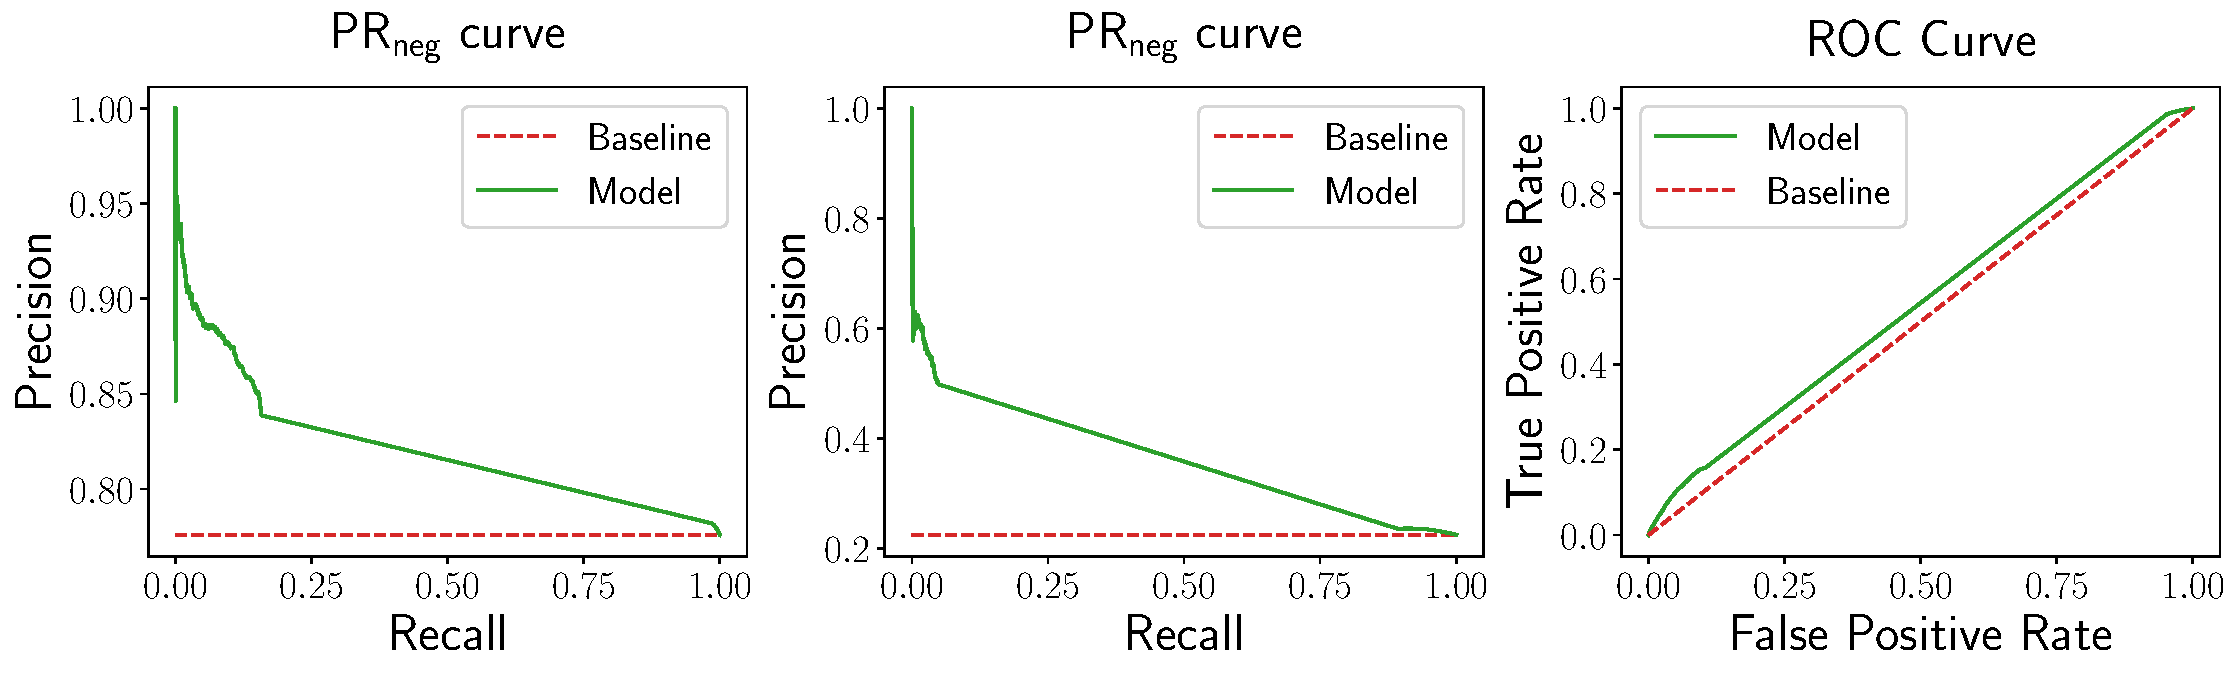
\includegraphics[width=\textwidth]{images/Logisitc Regression_test.pdf}
    \caption{Logistic Regression plots for test data}
    \label{fig:lr-test-plots}
\end{figure}



\begin{figure}[htp]
    \centering
    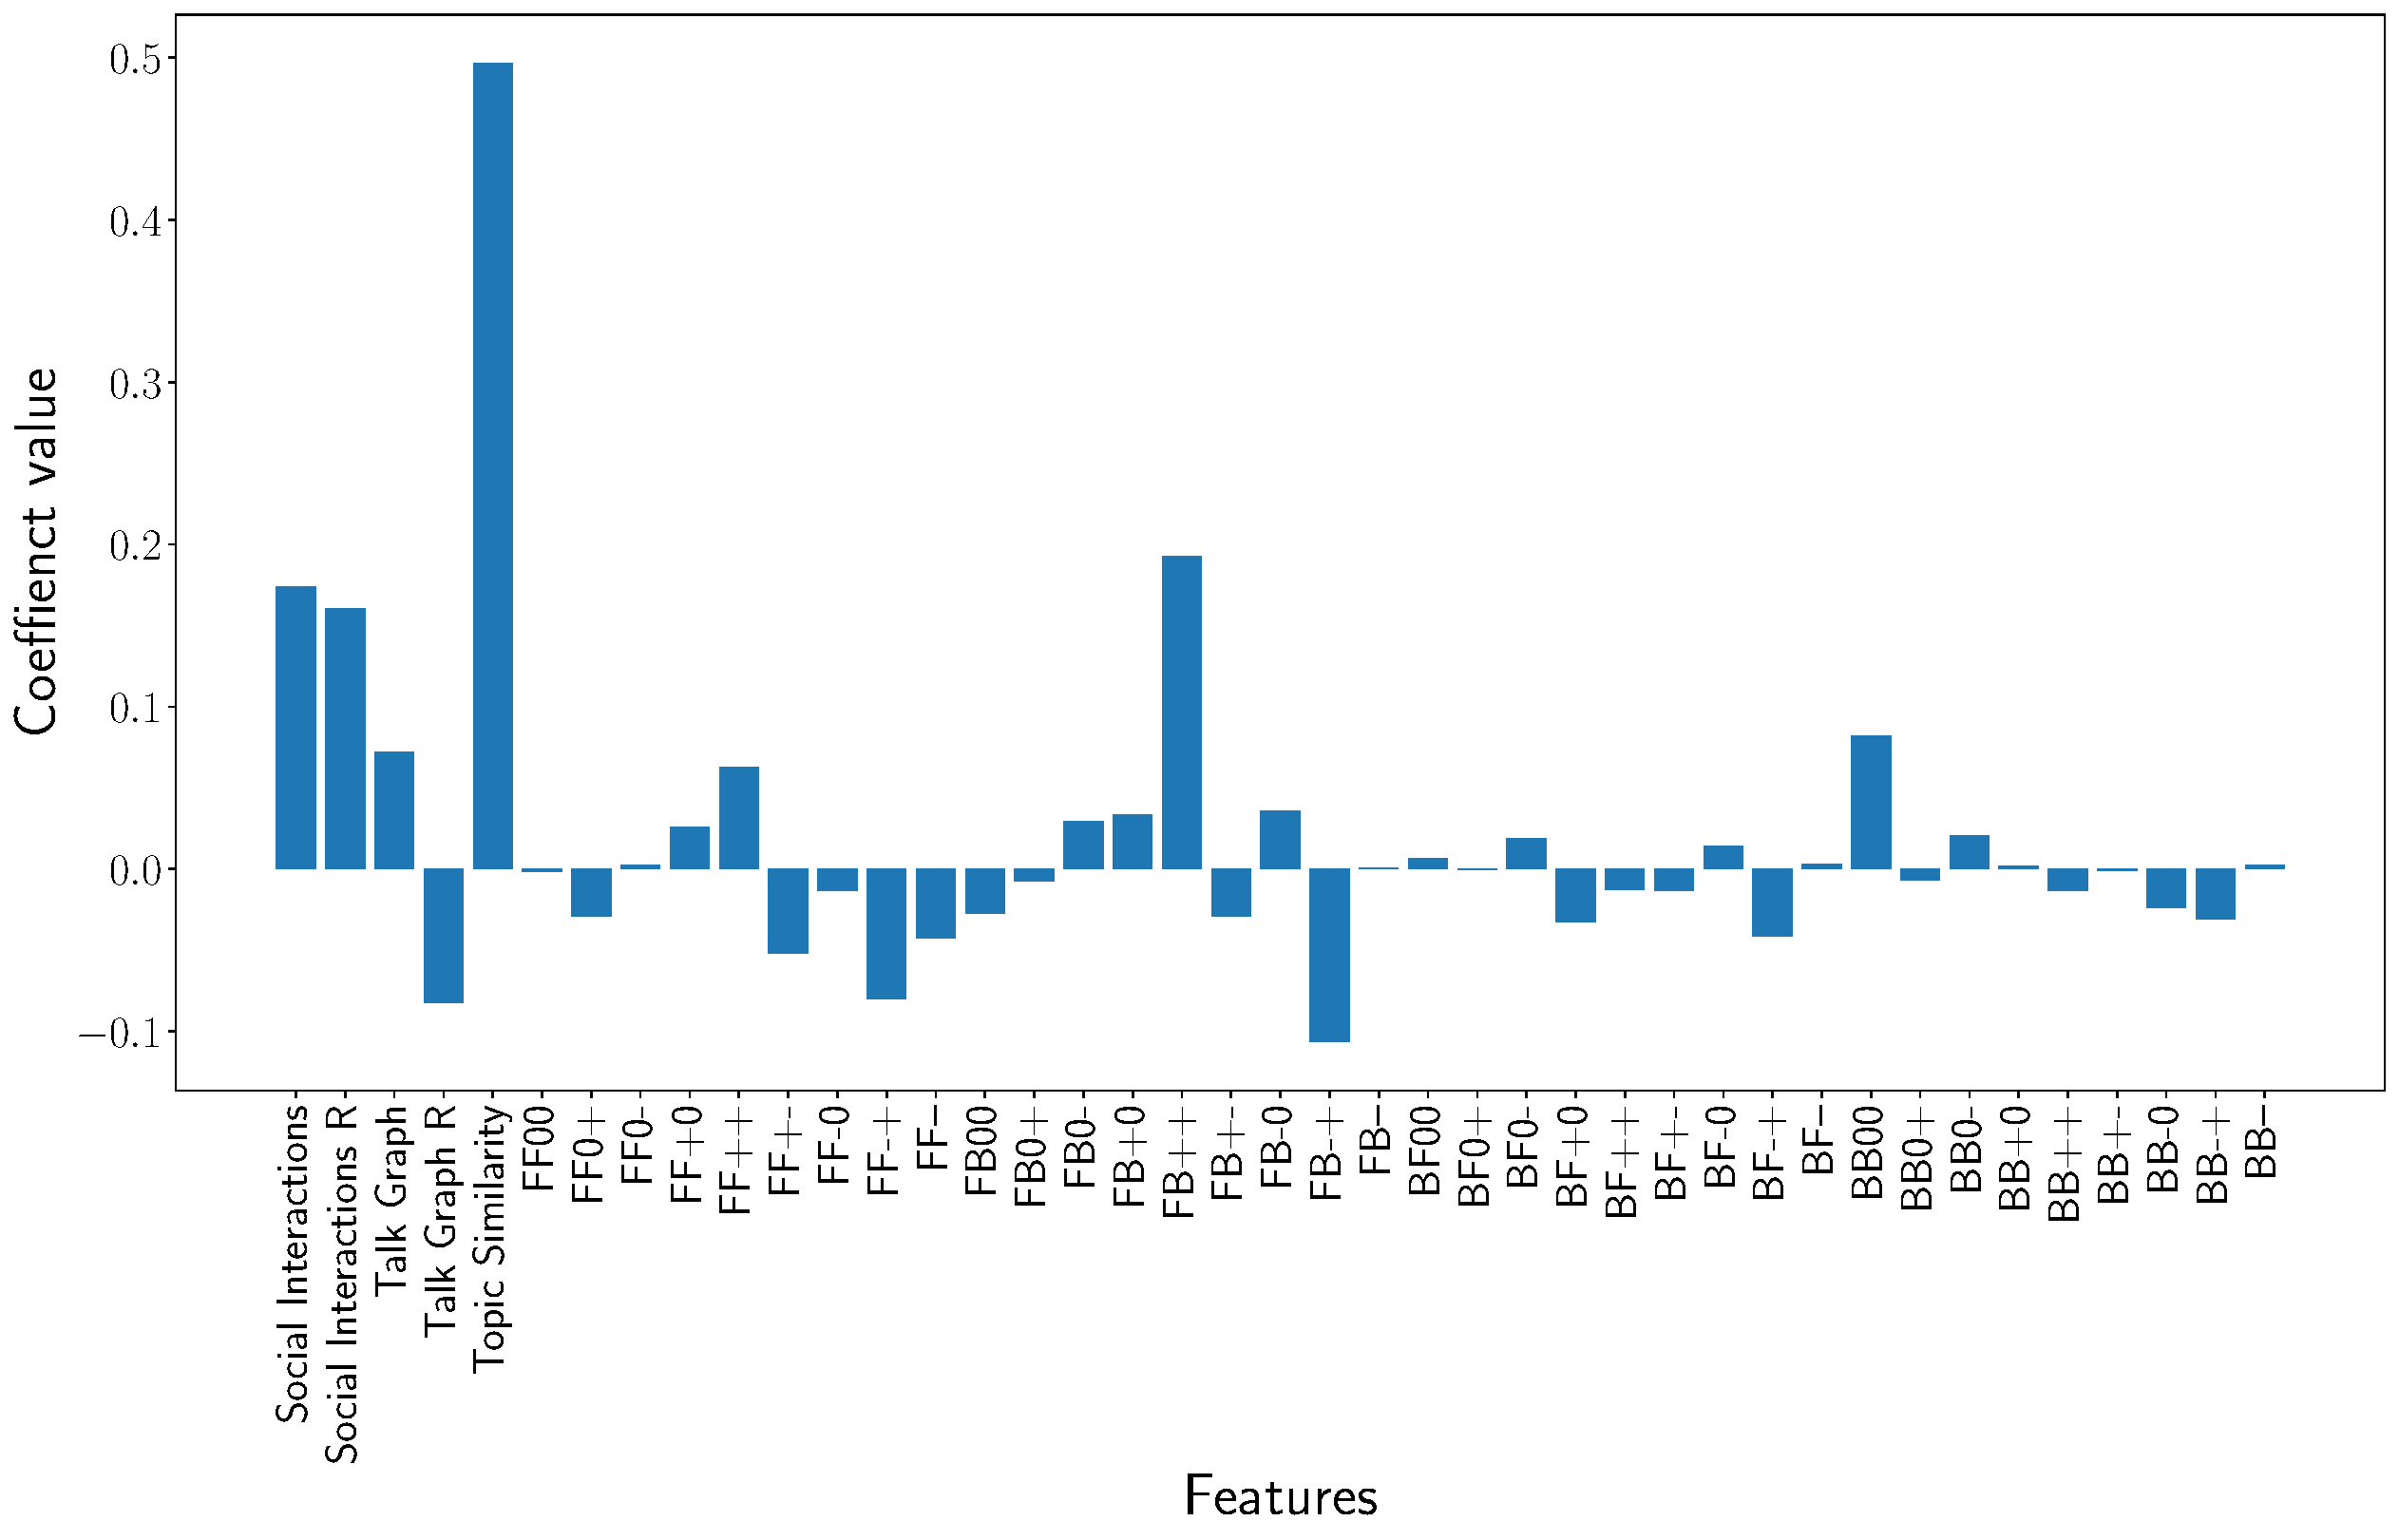
\includegraphics[width=\textwidth]{images/Logistic Regression_features.pdf}
    \caption{Feature importances for Logistic Regression model }
    \label{fig:lr-feature-importances}
\end{figure}
\begin{itemize}
    \item the description of the auxiliary graphs 
    \item Present results for LR model
    \item Show the ROC and PR curves
    \item Show the feature importances and discuss their relevance 
    \item Highlight the difficulty of predicting negative votes
\end{itemize}

\subsection{Iterative Model Results}
\begin{itemize}
    \item discuss how to compare the iterative model results
    \item Provide plots and table 
    \item Discuss the predictive power of the iterative model over the combination model
    \item Limitations and expansion of the graph combination model
\end{itemize}

\section{Complete \wikirfa Results}
\label{sec:complete-reults}
\begin{table}[htp]
    \centering
    \caption{Results of iterative models on the complete \wikirfa dataset}
    \label{tab:complete-results}
    \begin{tabular}{lccc}
        \toprule
        Model & AUC-ROC & \aucposPR  & \aucnegPR \\ 
        \midrule
        
        Baseline & 0.5 & 0.784& 0.216 \\

        Iterative Balance &  0.835 & 0.935 & 0.635 \\

        Iterative Status & 0.784 & 0.917 & 0.502 \\
        
        \bottomrule
        \end{tabular}
\end{table}

\begin{figure}[htp]
    \centering
    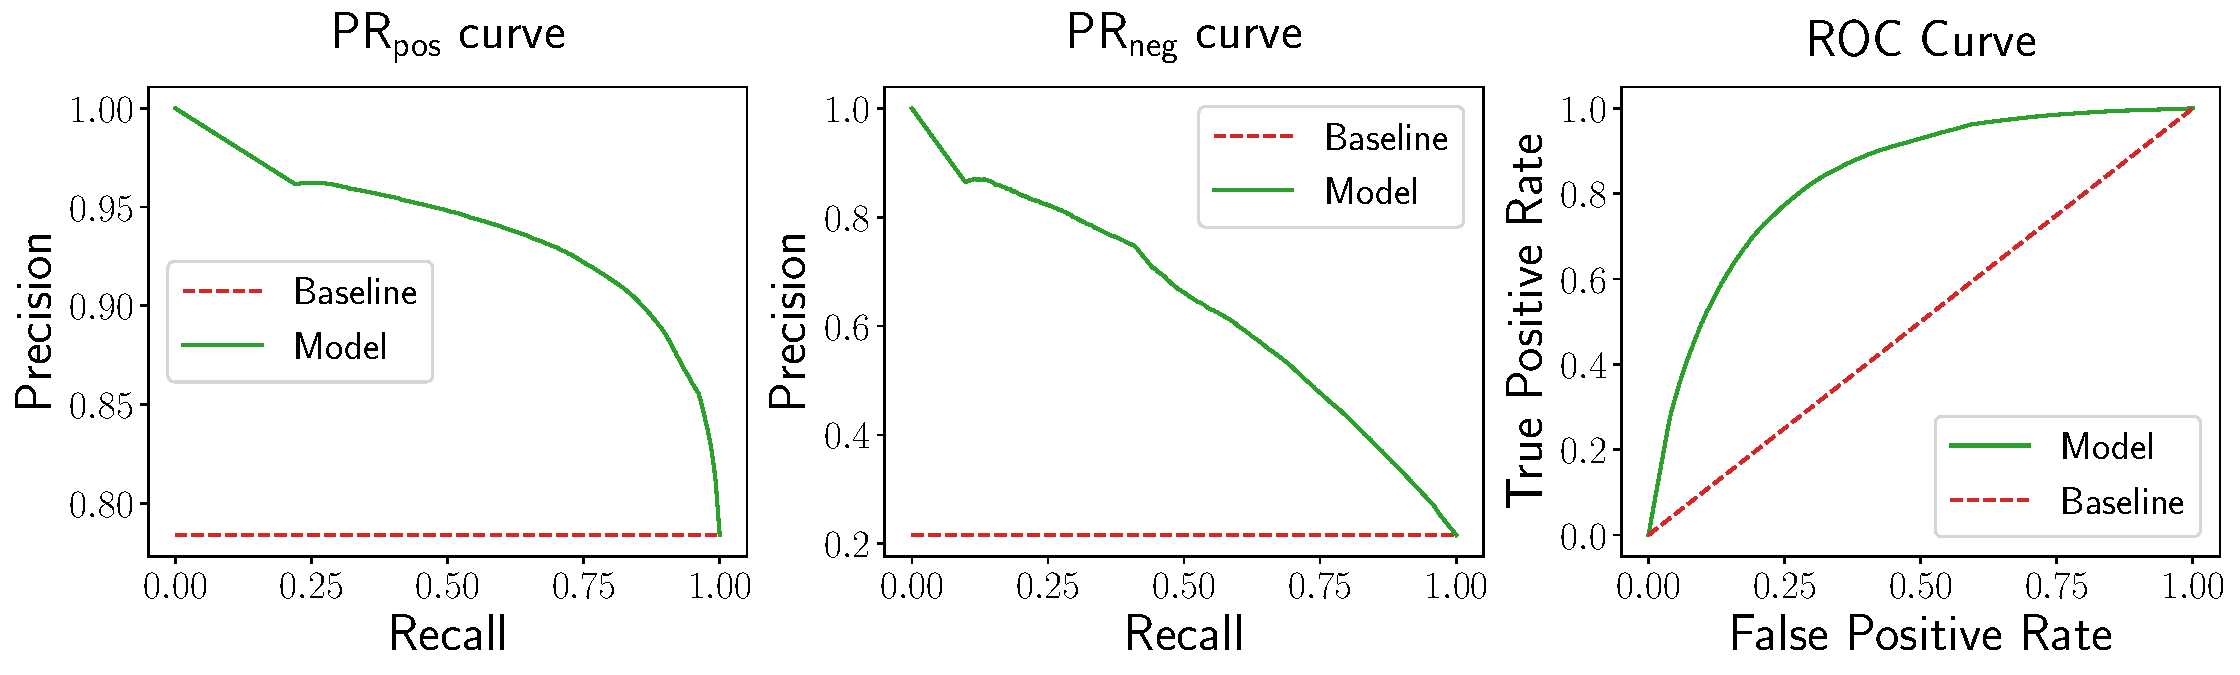
\includegraphics[width=\textwidth]{images/iterative_Balance.pdf}
    \caption{Plots for the Iterative Balance Model on the complete \wikirfa dataset}
    \label{fig:complete-iterative-balance}
\end{figure}

\begin{figure}[htp]
    \centering
    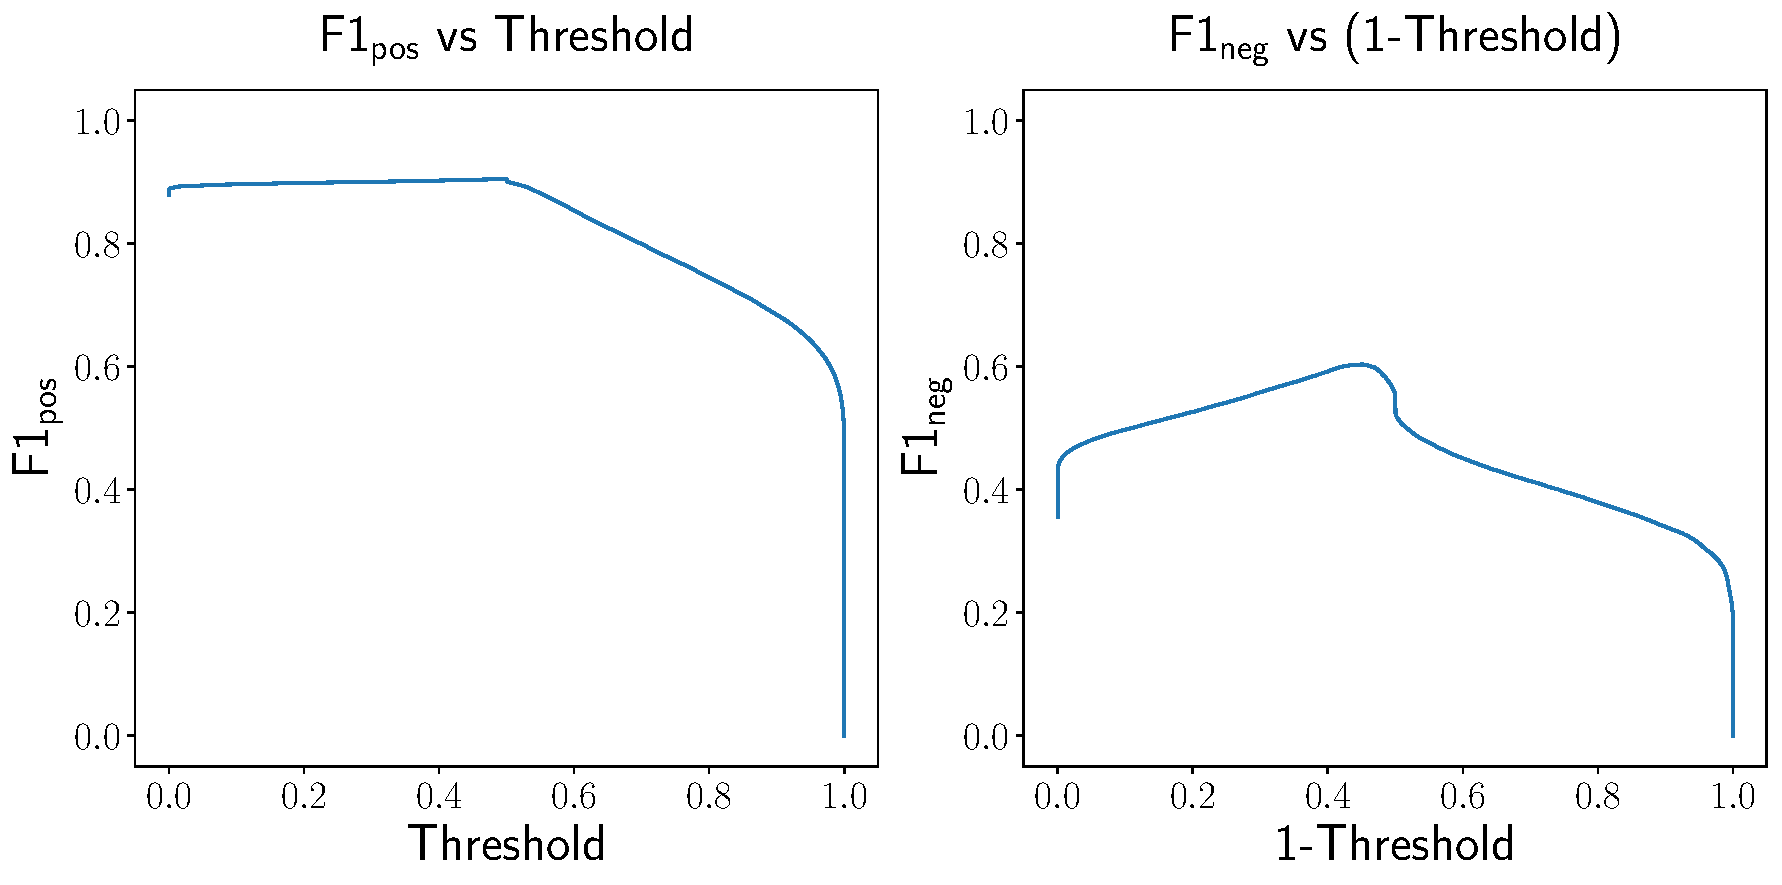
\includegraphics[width=0.75\textwidth]{images/iterative_Balance_f1.pdf}
    \caption{F1 score versus threshold plots for Iterative Balance Model}
    \label{fig:complete-iterative-balance-f1}
\end{figure}


\begin{figure}[htp]
    \centering
    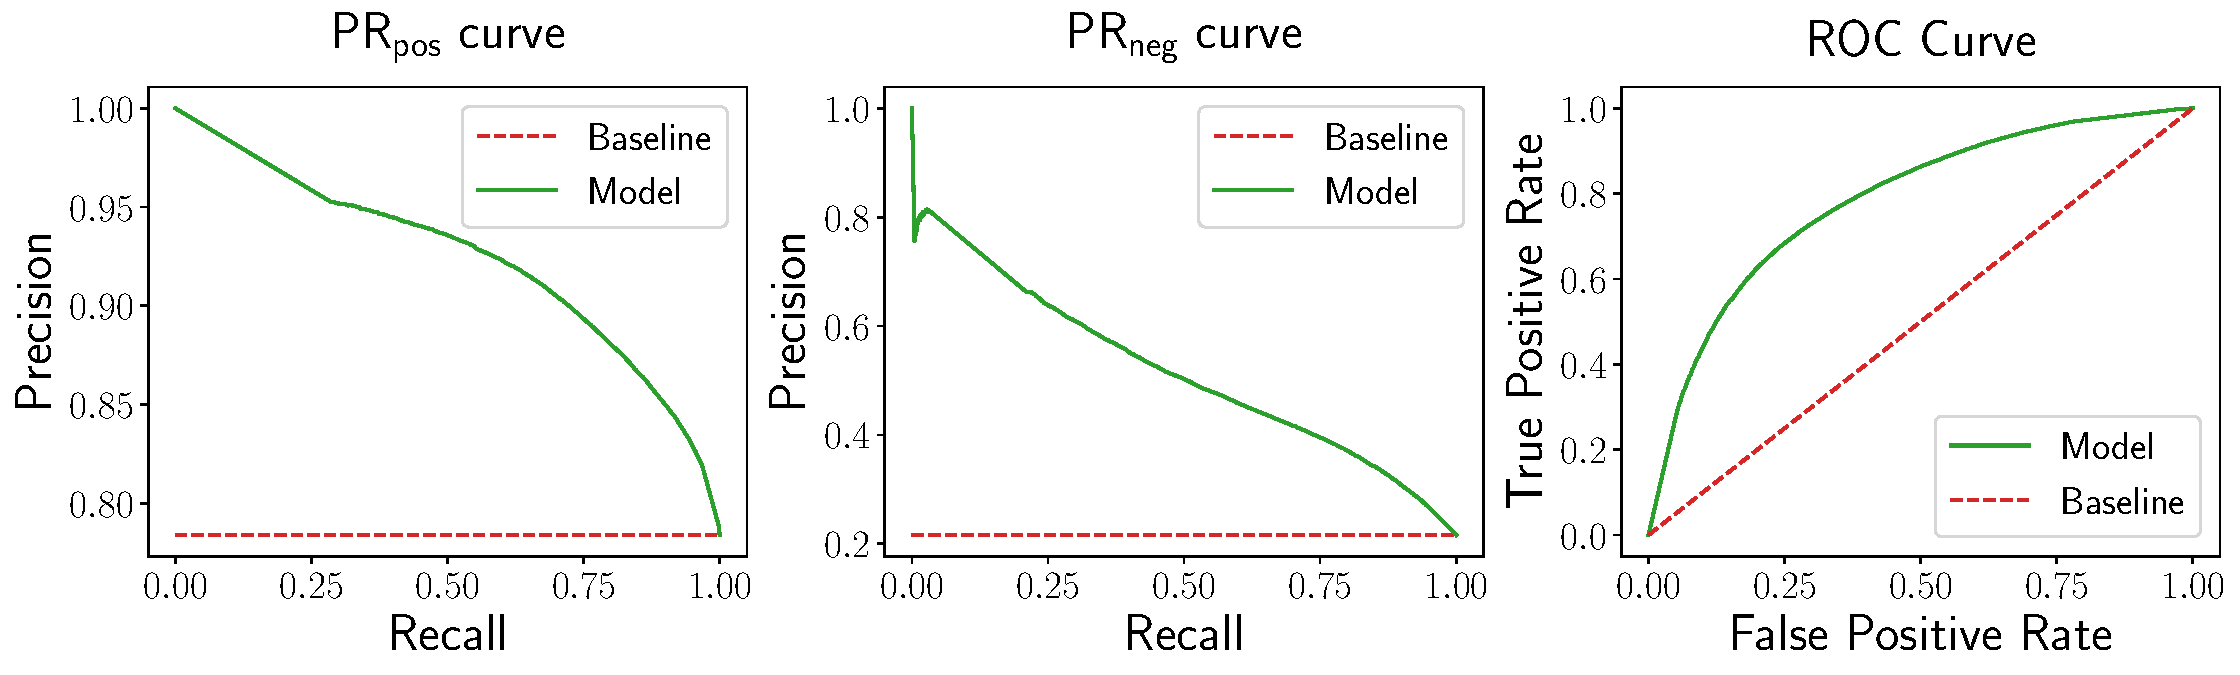
\includegraphics[width=\textwidth]{images/iterative_Status.pdf}
    \caption{Plots for the Iterative Status Model on the complete \wikirfa dataset}
    \label{fig:complete-iterative-status}
\end{figure}


\begin{figure}[htp]
    \centering
    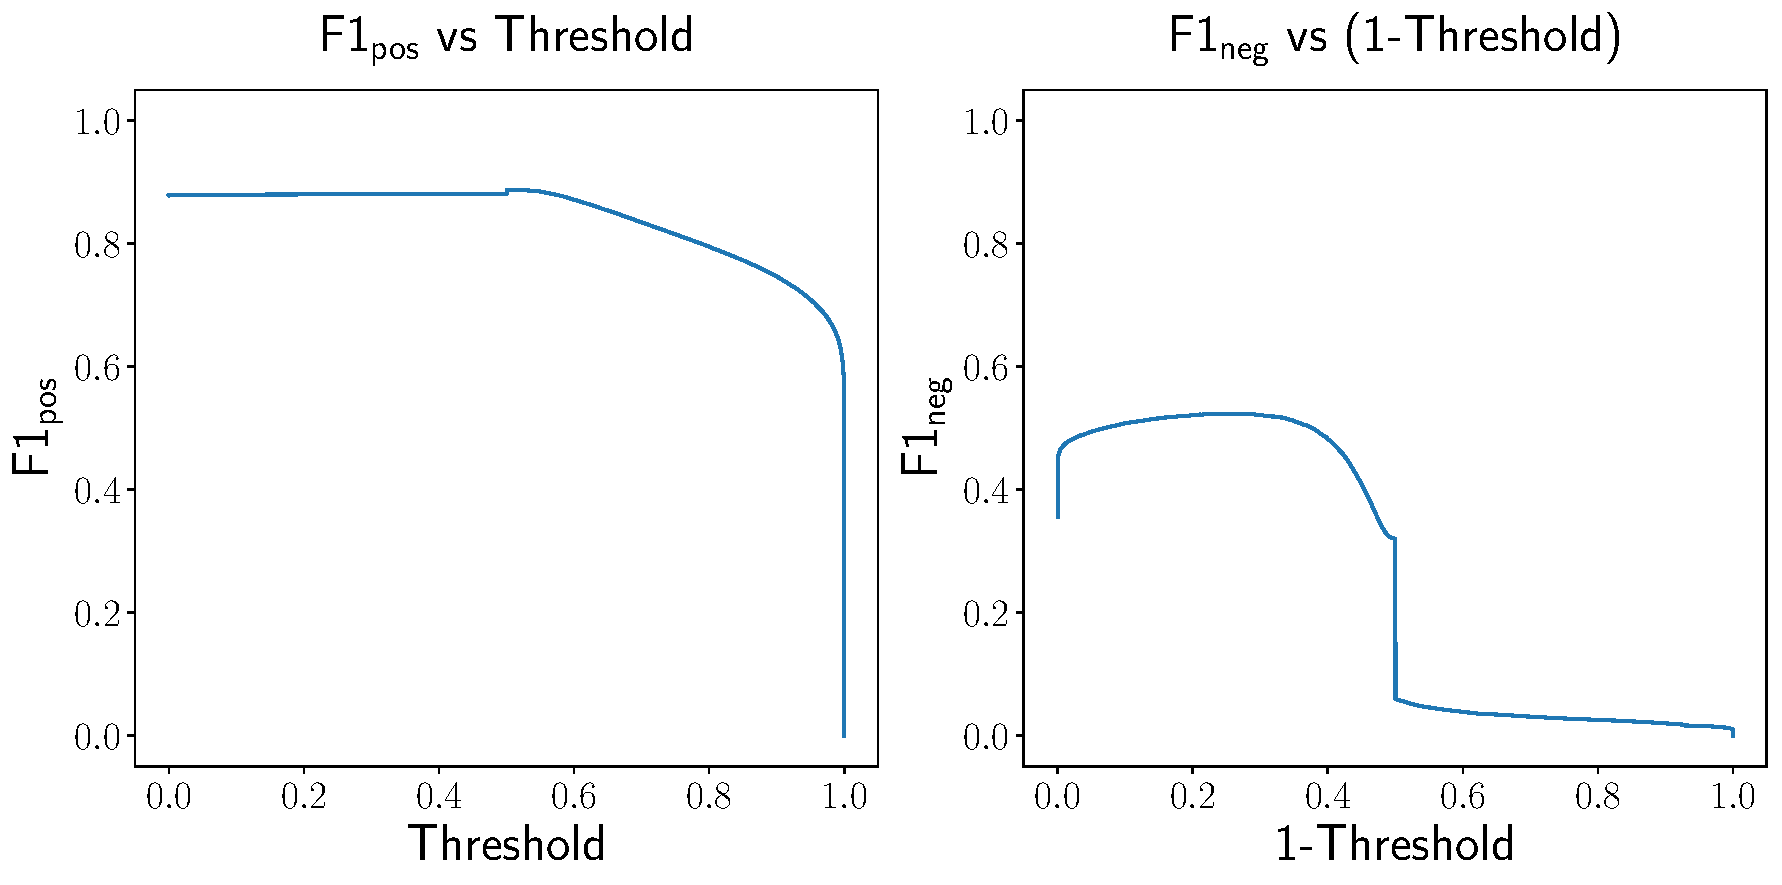
\includegraphics[width=0.75\textwidth]{images/iterative_Status_f1.pdf}
    \caption{F1 score versus threshold plots for Iterative Status Model}
    \label{fig:complete-iterative-status-f1}
\end{figure}



\begin{itemize}
    \item Present the Iterative Balance model results
    \item Discuss quality of predictions using evaluation metrics
    \item Explain the Iterative Status model results 
    \item Explain the selection of threshold and F1-score
\end{itemize}

\section{Voting Order Results}
\label{sec:voting-order-results}
\begin{table}[htp]
    \centering
    \caption{Results for different vote orderings for the failed RfA}
    \label{tab:fail-rfa}
    \begin{tabular}{llccc}
        \toprule
        Model & Vote Order & AUC-ROC & \aucposPR  & \aucnegPR \\ 
        \midrule
        
        Baseline & - & 0.5 & 0.52 & 0.479 \\
        \midrule
        
        \multirow{3}{*}{\shortstack[l]{Iterative\\ Balance}} & 
        Normal &  0.543 & 0.74 & 0.454 \\
        % \cmidrule{2-5}
        &Reversed & 0.74 & 0.868 & 0.572 \\
        % \cmidrule{2-5}
        & Random & 0.68 & 0.812 & 0.575 \\
        \midrule

        \multirow{3}{*}{\shortstack[l]{Iterative\\ Status}} & 
        Normal & 0.962 & 0.977 & 0.909 \\
        % \cmidrule{2-5}
        & Reversed & 0.930 & 0.965 & 0.806   \\
        % \cmidrule{2-5}
        & Random & 0.924 & 0.957 & 0.818 \\
        \bottomrule
        \end{tabular}
\end{table}

\begin{table}[htp]
    \centering
    \caption{Results for different vote orderings for the successful RfA}
    \label{tab:pass-rfa}
    \begin{tabular}{llccc}
        \toprule
        Model & Vote Order & ROC AUC & PR Positive  & Pr Negative \\ \midrule
        Baseline & - & 0.5 & 0.905 & 0.095 \\
        \midrule
        
        \multirow{3}{*}{\shortstack[l]{Iterative\\ Balance}} & 
        Normal &  0.9175 & 0.991 & 0.385 \\
        % \cmidrule{2-5}
        &Reversed & 0.720 & 0.972 & 0.142 \\
        % \cmidrule{2-5}
        & Random & 0.894 & 0.989 & 0.431 \\
        \midrule
        
        \multirow{3}{*}{\shortstack[l]{Iterative\\ Status}} & 
        Normal & 0.846 & 0.981 & 0.293 \\
        % \cmidrule{2-5}
        & Reversed & 0.895 & 0.99 & 0.29 \\
        % \cmidrule{2-5}
        & Random & 0.931 & 0.992 & 0.451 \\
        \bottomrule
        \end{tabular}
\end{table}


